
\section{Transparent without survivability}\label{ILP_Transp_Survivability}

\subsection{Model description}

To apply the ILP model we have to take into account the physical and logical topologies allowed by this mode of transport and the type of survivability. Based on section \ref{transparent} we can conclude that the topologies are different and the following figures can be confirmed.\\

\begin{figure}[h!]
\centering
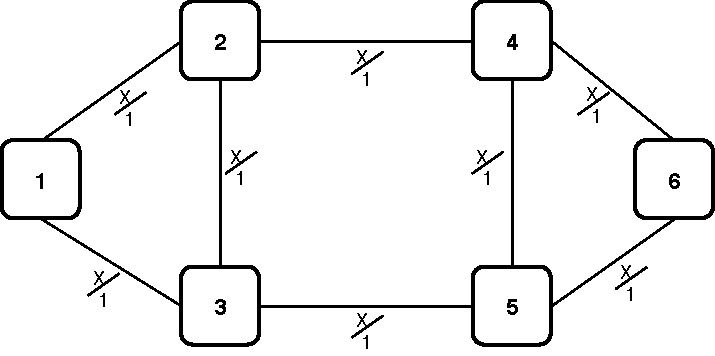
\includegraphics[width=11cm]{sdf/ilp/transparent_survivability/figures/allowed_physical_topology}
\caption{Transparent without survivability: allowed physical topology. The allowed physical topology is defined by the duct and sites in the field. It is assumed that each duct supports up to 1 bidirectional transmission system and each site supports up to 1 node.}
\label{allowed2_physical_low}
\end{figure}

\vspace{15pt}
\begin{figure}[h!]
\centering
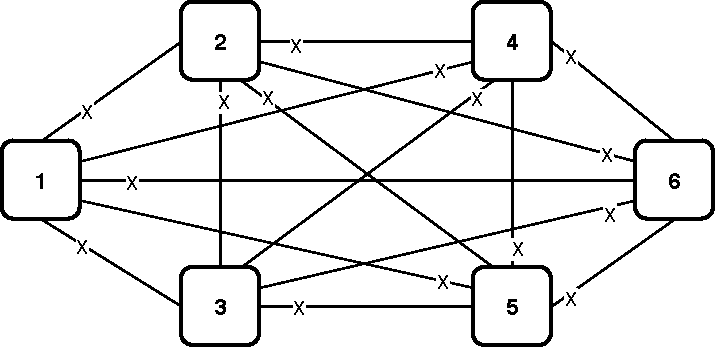
\includegraphics[width=11cm]{sdf/ilp/transparent_survivability/figures/allowed_optical_topology}
\caption{Transparent without survivability: allowed optical topology. The allowed optical topology is defined by the transport mode. It is assumed that each connections between demands supports up to 100 lightpaths.}
\label{allowed2_optical_low}
\end{figure}

Now taking this into consideration and based on the specific constraints of the transparent mode without survivability it is possible to define the ILP model \cite{aularui}.\\

The objective function, to be minimized, is the expression \ref{Capex}, i.e.,

\begin{equation*}
  minimize \qquad \Big\{ \quad C_C \quad \Big\}
\end{equation*}

$subject$ $to$
\begin{equation}
\sum_{c=1}^{C} (B\left(c\right) D_{odc}) \leq \tau \lambda_{od} \qquad \qquad \qquad \qquad \qquad \qquad \qquad \qquad \qquad
\forall(o,d) : o < d
\label{ILPTransp0_surv}
\end{equation}
\noindent
Constraint \ref{ILPTransp0_surv} is considered grooming constraint and for this model the grooming can be done before routing since the traffic is aggregated just for demands between the same nodes, thus not depending on the routes. The variable $\tau$ is always 100 Gbits/s.

\begin{equation}
\sum_{j=1\textbackslash \{o\}}^{N} f_{ij}^{od} = \lambda_{od}  \qquad \qquad \qquad \qquad \qquad \qquad \qquad \qquad
\forall(o,d) : o < d, \forall i: i = o
\label{ILPTransp1_surv}
\end{equation}
\noindent
Constraint \ref{ILPTransp1_surv} is equal to the constraint \ref{ILPOpaque1_CAPEX} assuming that Z is equal to the number of optical channels between demand $(o,d)$.

\begin{equation}
\sum_{j=1\textbackslash \{o\}}^{N} f_{ij}^{od} = \sum_{j=1\textbackslash \{d\}}^{N} f_{ji}^{od} \qquad \qquad \qquad \qquad \qquad \qquad
\forall(o,d) : o < d, \forall i: i \neq o,d
\label{ILPTransp2_surv}
\end{equation}
\noindent
Constraint \ref{ILPTransp2_surv} is equal to the constraint \ref{ILPOpaque2_CAPEX}.

\begin{equation}
\sum_{j=1\textbackslash \{d\}}^{N} f_{ji}^{od} = \lambda_{od}  \qquad \qquad \qquad \qquad \qquad \qquad \qquad \qquad
\forall(o,d) : o < d, \forall i: i = d
\label{ILPTransp3_surv}
\end{equation}
\noindent
Constraint \ref{ILPTransp3_surv} is equal to the constraint \ref{ILPOpaque3_CAPEX} assuming that Z is equal to the number of optical channels between demand $(o,d)$.

\begin{equation}
\sum_{o=1}^{N} \sum_{d=o+1}^{N} \left(f_{ij}^{od} + f_{ji}^{od}\right) \leq K_{ij} G_{ij} L_{ij} \qquad \qquad \qquad \qquad \qquad \qquad
\forall(i,j) : i < j
\label{ILPTransp4_surv}
\end{equation}
\noindent
Constraint \ref{ILPTransp4_surv} answers the capacity constraint problem. Then, total flows must be less or equal to the capacity of network links. For any situation the maximum number of optical channels supported by each transmission system is 100, i.e., $K_{ij}$ = 100.

\begin{equation}
f_{ij}^{od} , f_{ji}^{od} , \lambda_{od} \in \mathbb{N}   \qquad \qquad \qquad \qquad \qquad \qquad \qquad \qquad
\forall(i,j) : i < j, \forall(o,d) : o < d
\label{ILPTransp5_surv}
\end{equation}
\noindent
Last constraint define the total number of flows and the number of optical channels must be a counting number.

\subsection{Result description}

\textbf{Low Traffic Scenario:}\\

In a first phase, we will show the resulting physical and optical topology. These topologies are based on the allowed topologies referred to in the model description and also taking into account the logical topology for all ODUs mentioned in the section \ref{low_scenario}.

\begin{figure}[h!]
\centering
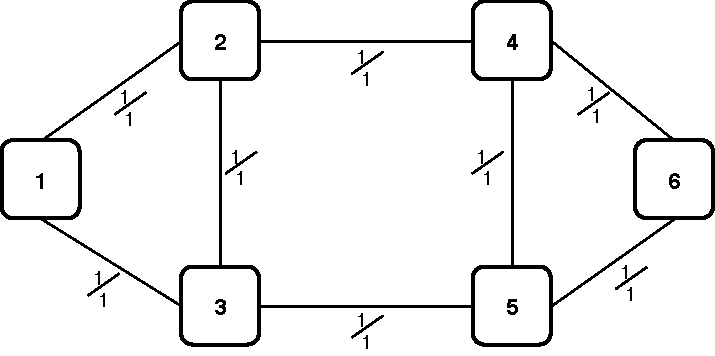
\includegraphics[width=11cm]{sdf/ilp/transparent_survivability/figures/physical_topology}
\caption{Transparent without survivability in low scenario: physical topology after dimensioning.}
\label{physical2_low}
\end{figure}

\newpage
\begin{figure}[h!]
\centering
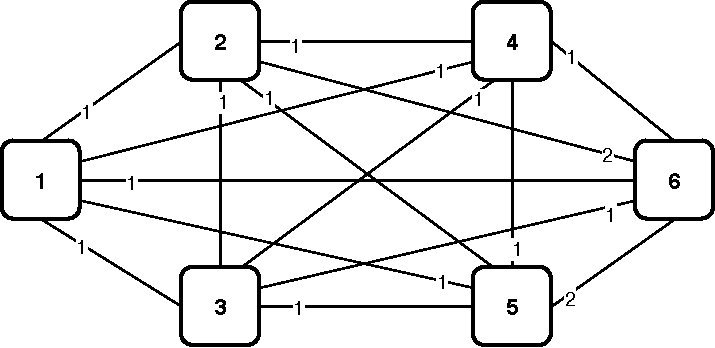
\includegraphics[width=11cm]{sdf/ilp/transparent_survivability/figures/optical_topology_low}
\caption{Transparent without survivability in low scenario: optical topology after dimensioning.}
\label{optical2_low}
\end{figure}

In table \ref{link_transp_surv_ref_low} we can see the number of optical channels calculated using \ref{Capex_Link} and \ref{ILPOpaque_CAPEX} and the number of amplifiers for each link calculated using \ref{Capex_amplifiers}.

\begin{table}[h!]
\centering
\begin{tabular}{|| c | c | c ||}
 \hline
 \multicolumn{3}{|| c ||}{Information regarding links} \\
 \hline
 \hline
 Bidirectional Link & Optical Channels & Amplifiers\\
 \hline
 Node 1 <-> Node 2 & 3 & 4 \\
 Node 1 <-> Node 3 & 2 & 6 \\
 Node 2 <-> Node 3 & 3 & 0 \\
 Node 2 <-> Node 4 & 6 & 6 \\
 Node 3 <-> Node 5 & 4 & 8 \\
 Node 4 <-> Node 5 & 1 & 1 \\
 Node 4 <-> Node 6 & 4 & 7 \\
 Node 5 <-> Node 6 & 3 & 3 \\
 \hline
\end{tabular}
\caption{Table with information regarding links for transparent mode without survivability in low scenario.}
\label{link_transp_surv_ref_low}
\end{table}

In table \ref{node_transp_surv_ref_low} we can see the number of line ports and add ports using \ref{OXC_poxc_transparent} the number of long-reach transponders using \ref{EXC_pexc2_transparent} and the number of tributary ports using \ref{EXC_pexc1_transparent}.

\begin{table}[h!]
\centering
\begin{tabular}{|| c | c | c | c | c | c ||}
 \hline
 \multicolumn{6}{|| c ||}{Information regarding nodes} \\
 \hline
 \hline
 \multicolumn{2}{|| c |}{ } & \multicolumn{2}{ c |}{Electrical part} & \multicolumn{2}{ c ||}{Optical part} \\
 \hline
 Node & Resulting Nodal Degree & Tributary Ports & LR Transponders & Add Ports & Line Ports\\
 \hline
 1 & 2 & 29 & 5 & 5 & 5 \\
 2 & 3 & 23 & 6 & 6 & 12 \\
 3 & 3 & 18 & 5 & 5 & 9 \\
 4 & 3 & 20 & 5 & 5 & 11 \\
 5 & 3 & 24 & 6 & 6 & 8 \\
 6 & 2 & 22 & 7 & 7 & 7 \\
\hline
\end{tabular}
\caption{Table with information regarding nodes for transparent mode without survivability in low scenario.}
\label{node_transp_surv_ref_low}
\end{table}
\newpage
Through the information obtained previously on the nodes we can now create tables with detailed information about each node. In each table mentioned below we can see how many ports are connected to a given node and its bit rate, the number os long-reach transponders and how many ports are assigned to each different bit rate.\\

\begin{table}[h!]
\centering
\begin{tabular}{|| c | c | c ||}
 \hline
 \multicolumn{3}{|| c ||}{Detailed description of Node 1} \\
 \hline
 \hline
 Electrical part & Number of total demands & Bit rate \\
 \hline
\multirow{3}{*}{29 tributary ports} & 13 & ODU0 \\
 & 13 & ODU1 \\
 & 3 & ODU2 \\
 \hline
  & Node<--Optical Channels-->Node & Bit rate \\
  \hline
\multirow{5}{*}{5 LR Transponders} & 1  <---- 1 ---->  2 & \multirow{5}{*}{100 Gbits/s} \\
  & 1  <---- 1 ---->  3 & \\
  & 1  <---- 1 ---->  4 & \\
  & 1  <---- 1 ---->  5 & \\
  & 1  <---- 1 ---->  6 & \\
 \hline
 \hline
 Optical part & Node<--Optical Channels-->Node & Bit rate \\
 \hline
 \multirow{5}{*}{5 add ports} & 1  <---- 1 ---->  2 & \multirow{10}{*}{100 Gbits/s} \\
  & 1  <---- 1 ---->  3 & \\
  & 1  <---- 1 ---->  4 & \\
  & 1  <---- 1 ---->  5 & \\
  & 1  <---- 1 ---->  6 & \\ \cline{1-2}
 \multirow{5}{*}{5 line ports} & 1  <---- 1 ---->  2 & \\
  & 1  <---- 1 ---->  3 & \\
  & 1  <---- 1 ---->  4 & \\
  & 1  <---- 1 ---->  5 & \\
  & 1  <---- 1 ---->  6 & \\
\hline
\end{tabular}
\caption{Transparent without survivability in low scenario: detailed description of node 1. The number of demands is distributed to the various destination nodes, this distribution can be observed in section \ref{low_scenario}. Regarding the number of line ports when this node is equal to the source, it means that add ports are used, otherwise it means that through ports are used. In this node as we can see there are no through ports.}
\end{table}

\newpage
\begin{table}[h!]
\centering
\begin{tabular}{|| c | c | c ||}
 \hline
 \multicolumn{3}{|| c ||}{Detailed description of Node 2} \\
 \hline
 \hline
 Electrical part & Number of total demands & Bit rate \\ \hline
\multirow{5}{*}{23 tributary ports} & 11 & ODU0 \\
 & 7 & ODU1 \\
 & 2 & ODU2 \\
 & 2 & ODU3 \\
 & 1 & ODU4 \\
 \hline
  & Node<--Optical Channels-->Node & Bit rate \\
  \hline
\multirow{5}{*}{6 LR Transponders} & 2  <---- 1 ---->  1 & \multirow{5}{*}{100 Gbits/s} \\
  & 2  <---- 1 ---->  3 & \\
  & 2  <---- 1 ---->  4 & \\
  & 2  <---- 1 ---->  5 & \\
  & 2  <---- 2 ---->  6 & \\
 \hline
 \hline
 Optical part & Node<--Optical Channels-->Node & Bit rate \\
 \hline
 \multirow{5}{*}{6 add ports} & 2  <---- 1 ---->  1 & \multirow{13}{*}{100 Gbits/s} \\
  & 2  <---- 1 ---->  3 & \\
  & 2  <---- 1 ---->  4 & \\
  & 2  <---- 1 ---->  5 & \\
  & 2  <---- 2 ---->  6 & \\ \cline{1-2}
 \multirow{8}{*}{12 line ports} & 2  <---- 1 ---->  1 & \\
  & 2  <---- 1 ---->  3 & \\
  & 2  <---- 1 ---->  4 & \\
  & 2  <---- 1 ---->  5 & \\
  & 2  <---- 2 ---->  6 & \\
  & 1  <---- 1 ---->  4 & \\
  & 1  <---- 1 ---->  6 & \\
  & 3  <---- 1 ---->  4 & \\
\hline
\end{tabular}
\caption{Transparent without survivability in low scenario: detailed description of node 2. The number of demands is distributed to the various destination nodes, this distribution can be observed in section \ref{low_scenario}. Regarding the number of line ports when this node is equal to the source, it means that add ports are used, otherwise it means that through ports are used. In the latter the number of ports is double the number of optical channels.}
\end{table}

\newpage
\begin{table}[h!]
\centering
\begin{tabular}{|| c | c | c ||}
 \hline
 \multicolumn{3}{|| c ||}{Detailed description of Node 3} \\
 \hline
 \hline
 Electrical part & Number of total demands & Bit rate \\
 \hline
 \multirow{4}{*}{18 tributary ports} & 7 & ODU0 \\
 & 6 & ODU1\\
 & 3 & ODU2\\
 & 2 & ODU3\\
 \hline
  & Node<--Optical Channels-->Node & Bit rate \\ \hline
 \multirow{5}{*}{5 LR Transponders} & 3  <---- 1 ---->  1 & \multirow{5}{*}{100 Gbits/s} \\
  & 3  <---- 1 ---->  2 & \\
  & 3  <---- 1 ---->  4 & \\
  & 3  <---- 1 ---->  5 & \\
  & 3  <---- 1 ---->  6 & \\
 \hline
 \hline
 Optical part & Node<--Optical Channels-->Node & Bit rate \\
 \hline
 \multirow{5}{*}{5 add ports} & 3  <---- 1 ---->  1 & \multirow{12}{*}{100 Gbits/s} \\
  & 3  <---- 1 ---->  2 & \\
  & 3  <---- 1 ---->  4 & \\
  & 3  <---- 1 ---->  5 & \\
  & 3  <---- 1 ---->  6 & \\ \cline{1-2}
 \multirow{7}{*}{9 line ports} & 3  <---- 1 ---->  1 & \\
  & 3  <---- 1 ---->  2 & \\
  & 3  <---- 1 ---->  4 & \\
  & 3  <---- 1 ---->  5 & \\
  & 3  <---- 1 ---->  6 & \\
  & 1  <---- 1 ---->  5 & \\
  & 2  <---- 1 ---->  5 & \\
\hline
\end{tabular}
\caption{Transparent without survivability in low scenario: detailed description of node 3. The number of demands is distributed to the various destination nodes, this distribution can be observed in section \ref{low_scenario}. Regarding the number of line ports when this node is equal to the source, it means that add ports are used, otherwise it means that through ports are used. In the latter the number of ports is double the number of optical channels.}
\end{table}

\newpage
\begin{table}[h!]
\centering
\begin{tabular}{|| c | c | c ||}
 \hline
 \multicolumn{3}{|| c ||}{Detailed description of Node 4} \\
 \hline
 \hline
 Electrical part & Number of total demands & Bit rate \\ \hline
\multirow{3}{*}{20 tributary ports} & 7 & ODU0 \\
 & 10 & ODU1 \\
 & 3 & ODU2 \\
 \hline
  & Node<--Optical Channels-->Node & Bit rate \\ \hline
 \multirow{5}{*}{5 LR Transponders} & 4  <---- 1 ---->  1 & \multirow{5}{*}{100 Gbits/s} \\
  & 4  <---- 1 ---->  2 & \\
  & 4  <---- 1 ---->  3 & \\
  & 4  <---- 1 ---->  5 & \\
  & 4  <---- 1 ---->  6 & \\
 \hline
 \hline
 Optical part & Node<--Optical Channels-->Node & Bit rate \\
 \hline
 \multirow{5}{*}{5 add ports} & 4  <---- 1 ---->  1 & \multirow{12}{*}{100 Gbits/s} \\
  & 4  <---- 1 ---->  2 & \\
  & 4  <---- 1 ---->  3 & \\
  & 4  <---- 1 ---->  5 & \\
  & 4  <---- 1 ---->  6 & \\ \cline{1-2}
 \multirow{7}{*}{11 line ports} & 4  <---- 1 ---->  1 & \\
  & 4  <---- 1 ---->  2 & \\
  & 4  <---- 1 ---->  3 & \\
  & 4  <---- 1 ---->  5 & \\
  & 4  <---- 1 ---->  6 & \\
  & 1  <---- 1 ---->  6 & \\
  & 2  <---- 2 ---->  6 & \\
\hline
\end{tabular}
\caption{Transparent without survivability in low scenario: detailed description of node 4. The number of demands is distributed to the various destination nodes, this distribution can be observed in section \ref{low_scenario}. Regarding the number of line ports when this node is equal to the source, it means that add ports are used, otherwise it means that through ports are used. In the latter the number of ports is double the number of optical channels.}
\end{table}

\newpage
\begin{table}[h!]
\centering
\begin{tabular}{|| c | c | c ||}
 \hline
 \multicolumn{3}{|| c ||}{Detailed description of Node 5} \\
 \hline
 \hline
 Electrical part & Number of total demands & Bit rate \\ \hline
\multirow{5}{*}{24 tributary ports} & 14 & ODU0 \\
 & 4 & ODU1 \\
 & 4 & ODU2 \\
 & 1 & ODU3 \\
 & 1 & ODU4 \\
 \hline
  & Node<--Optical Channels-->Node & Bit rate \\ \hline
 \multirow{5}{*}{6 LR Transponders} & 5  <---- 1 ---->  1 & \multirow{5}{*}{100 Gbits/s} \\
  & 5  <---- 1 ---->  2 & \\
  & 5  <---- 1 ---->  3 & \\
  & 5  <---- 1 ---->  4 & \\
  & 5  <---- 2 ---->  6 & \\
 \hline
 \hline
 Optical part & Node<--Optical Channels-->Node & Bit rate \\
 \hline
 \multirow{5}{*}{6 add ports} & 5  <---- 1 ---->  1 & \multirow{11}{*}{100 Gbits/s} \\
  & 5  <---- 1 ---->  2 & \\
  & 5  <---- 1 ---->  3 & \\
  & 5  <---- 1 ---->  4 & \\
  & 5  <---- 2 ---->  6 & \\ \cline{1-2}
 \multirow{6}{*}{8 line ports} & 5  <---- 1 ---->  1 & \\
  & 5  <---- 1 ---->  2 & \\
  & 5  <---- 1 ---->  3 & \\
  & 5  <---- 1 ---->  4 & \\
  & 5  <---- 2 ---->  6 & \\
  & 3  <---- 1 ---->  6 &\\
\hline
\end{tabular}
\caption{Transparent without survivability in low scenario: detailed description of node 5. The number of demands is distributed to the various destination nodes, this distribution can be observed in section \ref{low_scenario}. Regarding the number of line ports when this node is equal to the source, it means that add ports are used, otherwise it means that through ports are used. In the latter the number of ports is double the number of optical channels.}
\end{table}

\newpage
\begin{table}[h!]
\centering
\begin{tabular}{|| c | c | c ||}
 \hline
 \multicolumn{3}{|| c ||}{Detailed description of Node 6} \\
 \hline
 \hline
 Electrical part & Number of total demands & Bit rate \\ \hline
\multirow{5}{*}{22 tributary ports} & 8 & ODU0 \\
 & 10 & ODU1 \\
 & 1 & ODU2 \\
 & 1 & ODU3 \\
 & 2 & ODU4 \\
 \hline
  & Node<--Optical Channels-->Node & Bit rate \\ \hline
 \multirow{5}{*}{7 LR Transponders} & 6  <---- 1 ---->  1 & \multirow{5}{*}{100 Gbits/s} \\
  & 6  <---- 2 ---->  2 & \\
  & 6  <---- 1 ---->  3 & \\
  & 6  <---- 1 ---->  4 & \\
  & 6  <---- 2 ---->  5 & \\
 \hline
 Optical part & Node<--Optical Channels-->Node & Bit rate \\
 \hline
 \multirow{5}{*}{7 add ports} & 6  <---- 1 ---->  1 & \multirow{10}{*}{100 Gbits/s} \\
  & 6  <---- 2 ---->  2 & \\
  & 6  <---- 1 ---->  3 & \\
  & 6  <---- 1 ---->  4 & \\
  & 6  <---- 2 ---->  5 & \\ \cline{1-2}
 \multirow{5}{*}{7 line ports} & 6  <---- 1 ---->  1 & \\
  & 6  <---- 2 ---->  2 & \\
  & 6  <---- 1 ---->  3 & \\
  & 6  <---- 1 ---->  4 & \\
  & 6  <---- 2 ---->  5 & \\
\hline
\end{tabular}
\caption{Transparent without survivability in low scenario: detailed description of node 6. The number of demands is distributed to the various destination nodes, this distribution can be observed in section \ref{low_scenario}. Regarding the number of line ports when this node is equal to the source, it means that add ports are used, otherwise it means that through ports are used.  In this node as we can see there are no through ports.}
\end{table}

\vspace{13pt}
Now, in next page, let's focus on the routing information in table \ref{path_transp_surv_ref_low}. These paths are bidirectional so the path from one node to another is the same path in the opposite direction.\\
\newpage
\begin{table}[h!]
\centering
\begin{tabular}{|| c | c | c | c | c | c | c | c ||}
 \hline
 \multicolumn{8}{|| c ||}{Routing} \\
 \hline
 \hline
 o & d & Links & ODU0 & ODU1 & ODU2 & ODU3 & ODU4 \\
 \hline
 1 & 2 & \{(1,2)\} & 5 & 2 & 1 & 0 & 0 \\ \hline
 1 & 3 & \{(1,3)\} & 1 & 4 & 1 & 0 & 0\\ \hline
 1 & 4 & \{(1,2),(2,4)\} & 3 & 2 & 1 & 0 & 0\\ \hline
 1 & 5 & \{(1,3),(3,5)\} & 1 & 0 & 0 & 0 & 0\\ \hline
 1 & 6 & \{(1,2),(2,4),(4,6)\} & 3 & 5 & 0 & 0 & 0\\ \hline
 2 & 3 & \{(2,3)\} & 0 & 0 & 0 & 1 & 0 \\ \hline
 2 & 4 & \{(2,4)\} & 1 & 3 & 0 & 0 & 0\\ \hline
 2 & 5 & \{(2,3),(3,5)\} & 5 & 1 & 1 & 0 & 0 \\ \hline
 2 & 6 & \{(2,4),(4,6)\} & 0 & 1 & 0 & 1 & 1 \\ \hline
 3 & 4 & \{(3,2),(2,4)\} & 1 & 1 & 1 & 0 & 0 \\ \hline
 3 & 5 & \{(3,5)\} & 4 & 1 & 1 & 1 & 0 \\ \hline
 3 & 6 & \{(3,5),(5,6)\} & 1 & 0 & 0 & 0 & 0\\ \hline
 4 & 5 & \{(4,5)\} & 1 & 1 & 1 & 0 & 0\\ \hline
 4 & 6 & \{(4,6)\} & 1 & 3 & 0 & 0 & 0\\ \hline
 5 & 6 & \{(5,6)\} & 3 & 1 & 1 & 0 & 1\\
 \hline
\end{tabular}
\caption{Transparent without survivability in low scenario: description of routing.}
\label{path_transp_surv_ref_low}
\end{table}

Finally through table \ref{scripttransp_surv_ref_low} we can see the CAPEX result for this model. This value is obtained using equation \ref{ILPOpaque_CAPEX} and all of the constraints mentioned above.\\

\begin{table}[h!]
\centering
\begin{tabular}{||c|c|c|c|c|c|c||}
 \hline
 \multicolumn{7}{||c||}{CAPEX of the Network} \\
 \hline
 \hline
 \multicolumn{3}{||c|}{} & Quantity & Unit Price & Cost & Total \\
 \hline
 \multirow{3}{*}{\makecell{Link \\ Cost}} &\multicolumn{2}{c|}{OLTs}&16&15 000 \euro&240 000 \euro&\multirow{3}{*}{26 520 000 \euro} \\ \cline{2-6}
 & \multicolumn{2}{c|}{100 Gbits/s Transceivers}&52&5 000 \euro/Gbit/s&26 000 000 \euro& \\ \cline{2-6}
 & \multicolumn{2}{c|}{Amplifiers}&70&4 000 \euro&280 000 \euro& \\
 \hline
 \multirow{10}{*}{\makecell{Node \\ Cost}} &\multirow{7}{*}{Electrical}& EXCs & 6 & 10 000 \euro & 60 000 \euro & \multirow{10}{*}{3 797 590 \euro} \\ \cline{3-6}
 & &ODU0 Ports&60&10 \euro/port& 600 \euro & \\ \cline{3-6}
 & &ODU1 Ports&50&15 \euro/port& 750 \euro & \\ \cline{3-6}
 & &ODU2 Ports&16&30 \euro/port& 480 \euro & \\ \cline{3-6}
 & &ODU3 Ports&6&60 \euro/port& 360 \euro & \\ \cline{3-6}
 & &ODU4 Ports&4&100 \euro/port& 400 \euro & \\ \cline{3-6}
 & &Transponders&34&100 000 \euro/port&3 400 000 \euro& \\ \cline{2-6}
 & \multirow{3}{*}{Optical} & OXCs & 6 &20 000 \euro&120 000 \euro& \\ \cline{3-6}
 & &Line Ports& 52 & 2 500 \euro/port &130 000 \euro& \\ \cline{3-6}
 & &Add Ports& 34 & 2 500 \euro/port &85 000 \euro& \\
 \hline
 \multicolumn{6}{||c|}{Total Network Cost} & 30 317 590 \euro \\
\hline
\end{tabular}
\caption{Transparent without survivability in low scenario: detailed description of CAPEX for this scenario.}
\label{scripttransp_surv_ref_low}
\end{table}

\newpage
\textbf{Medium Traffic Scenario:}\\

In a first phase, we will show the resulting physical and optical topology. These topologies are based on the allowed topologies referred to in the model description and also taking into account the logical topology for all ODU's mentioned in the section \ref{medium_traffic_scenario}.\\

\begin{figure}[h!]
\centering
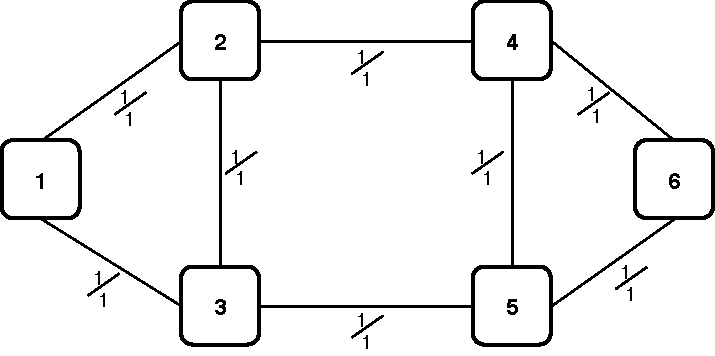
\includegraphics[width=11cm]{sdf/ilp/transparent_survivability/figures/physical_topology}
\caption{Transparent without survivability in medium scenario: physical topology after dimensioning.}
\label{physical2_medium}
\end{figure}

\vspace{15pt}
\begin{figure}[h!]
\centering
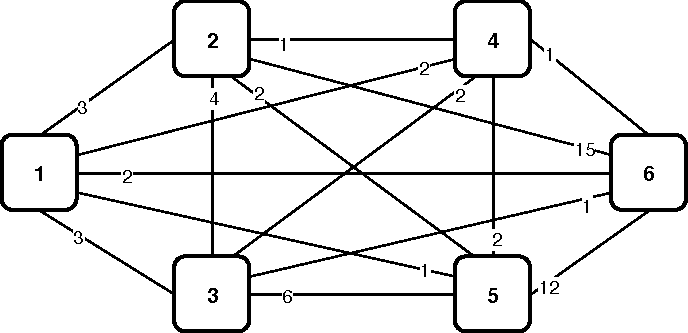
\includegraphics[width=11cm]{sdf/ilp/transparent_survivability/figures/optical_topology_medium}
\caption{Transparent without survivability in medium scenario: optical topology after dimensioning.}
\label{optical2_medium}
\end{figure}

\newpage
In table \ref{link_transp_surv_ref_medium} we can see the number of optical channels calculated using \ref{Capex_Link} and \ref{ILPOpaque_CAPEX} and the number of amplifiers for each link calculated using \ref{Capex_amplifiers}.\\

\begin{table}[h!]
\centering
\begin{tabular}{|| c | c | c ||}
 \hline
 \multicolumn{3}{|| c ||}{Information regarding links} \\
 \hline
 \hline
 Bidirectional Link & Optical Channels & Amplifiers\\
 \hline
 Node 1 <-> Node 2 & 7 & 4 \\
 Node 1 <-> Node 3 & 4 & 6 \\
 Node 2 <-> Node 3 & 8 & 0 \\
 Node 2 <-> Node 4 & 22 & 6 \\
 Node 3 <-> Node 5 & 10 & 8 \\
 Node 4 <-> Node 5 & 2 & 1 \\
 Node 4 <-> Node 6 & 18 & 7 \\
 Node 5 <-> Node 6 & 13 & 3 \\
 \hline
\end{tabular}
\caption{Table with information regarding links for transparent mode without survivability in medium scenario.}
\label{link_transp_surv_ref_medium}
\end{table}

In table \ref{node_transp_surv_ref_medium} we can see the number of line ports and add ports using \ref{OXC_poxc_transparent} the number of long-reach transponders using \ref{EXC_pexc2_transparent} and the number of tributary ports using \ref{EXC_pexc1_transparent}.\\

\begin{table}[h!]
\centering
\begin{tabular}{|| c | c | c | c | c | c ||}
 \hline
 \multicolumn{6}{|| c ||}{Information regarding nodes} \\
 \hline
 \hline
 \multicolumn{2}{|| c |}{ } & \multicolumn{2}{ c |}{Electrical part} & \multicolumn{2}{ c ||}{Optical part} \\
 \hline
 Node & Resulting Nodal Degree & Tributary Ports & LR Transponders & Add Ports & Line Ports\\
 \hline
 1 & 2 & 290 & 11 & 11 & 11 \\
 2 & 3 & 230 & 25 & 25 & 37 \\
 3 & 3 & 180 & 16 & 16 & 22 \\
 4 & 3 & 200 & 8 & 8 & 42 \\
 5 & 3 & 240 & 23 & 23 & 25 \\
 6 & 2 & 220 & 31 & 31 & 31 \\
\hline
\end{tabular}
\caption{Table with information regarding nodes for transparent mode without survivability in medium scenario.}
\label{node_transp_surv_ref_medium}
\end{table}

\newpage
Through the information obtained previously on the nodes we can now create tables with detailed information about each node. In each table mentioned below we can see how many ports are connected to a given node and its bit rate (in relation to the line ports and the add ports), the number of long-reach transponders and how many ports are assigned to each different bit rate (in relation to the tributary ports).\\

\begin{table}[h!]
\centering
\begin{tabular}{|| c | c | c ||}
 \hline
 \multicolumn{3}{|| c ||}{Detailed description of Node 1} \\
 \hline
 \hline
 Electrical part & Number of total demands & Bit rate \\ \hline
\multirow{3}{*}{290 tributary ports} & 130 & ODU0 \\
 & 130 & ODU1 \\
 & 30 & ODU2 \\
 \hline
  & Node<--Optical Channels-->Node & Bit rate \\ \hline
 \multirow{5}{*}{11 LR Transponders} & 1  <---- 3 ---->  2 & \multirow{5}{*}{100 Gbits/s} \\
  & 1  <---- 3 ---->  3 & \\
  & 1  <---- 2 ---->  4 & \\
  & 1  <---- 1 ---->  5 & \\
  & 1  <---- 2 ---->  6 & \\
 \hline
 \hline
 Optical part & Node<--Optical Channels-->Node & Bit rate \\
 \hline
 \multirow{5}{*}{11 add ports} & 1  <---- 3 ---->  2 & \multirow{10}{*}{100 Gbits/s} \\
  & 1  <---- 3 ---->  3 & \\
  & 1  <---- 2 ---->  4 & \\
  & 1  <---- 1 ---->  5 & \\
  & 1  <---- 2 ---->  6 & \\ \cline{1-2}
 \multirow{5}{*}{11 line ports} & 1  <---- 3 ---->  2 & \\
  & 1  <---- 3 ---->  3 & \\
  & 1  <---- 2 ---->  4 & \\
  & 1  <---- 1 ---->  5 & \\
  & 1  <---- 2 ---->  6 & \\
\hline
\end{tabular}
\caption{Transparent without survivability in medium scenario: detailed description of node 1. The number of demands is distributed to the various destination nodes, this distribution can be observed in section \ref{medium_traffic_scenario} . Regarding the number of line ports when this node is equal to the source, it means that add ports are used, otherwise it means that through ports are used.  In this node as we can see there are no through ports.}
\end{table}

\newpage
\begin{table}[h!]
\centering
\begin{tabular}{|| c | c | c ||}
 \hline
 \multicolumn{3}{|| c ||}{Detailed description of Node 2} \\
 \hline
 \hline
 Electrical part & Number of total demands & Bit rate \\ \hline
\multirow{5}{*}{230 tributary ports} & 110 & ODU0 \\
 & 70 & ODU1 \\
 & 20 & ODU2 \\
 & 20 & ODU3 \\
 & 10 & ODU4 \\
 \hline
  & Node<--Optical Channels-->Node & Bit rate \\
 \hline
 \multirow{5}{*}{25 LR Transponders} & 2  <---- 3 ---->  1 & \multirow{5}{*}{100 Gbits/s} \\
  & 2  <---- 4 ---->  3 & \\
  & 2  <---- 1 ---->  4 & \\
  & 2  <---- 2 ---->  5 & \\
  & 2  <---- 15 ---->  6 & \\
 \hline
 \hline
 Optical part & Node<--Optical Channels-->Node & Bit rate \\
 \hline
 \multirow{5}{*}{25 add ports} & 2  <---- 3 ---->  1 & \multirow{13}{*}{100 Gbits/s} \\
  & 2  <---- 4 ---->  3 & \\
  & 2  <---- 1 ---->  4 & \\
  & 2  <---- 2 ---->  5 & \\
  & 2  <---- 15 ---->  6 & \\ \cline{1-2}
 \multirow{8}{*}{37 line ports} & 2  <---- 3 ---->  1 & \\
  & 2  <---- 4 ---->  3 & \\
  & 2  <---- 1 ---->  4 & \\
  & 2  <---- 2 ---->  5 & \\
  & 2  <---- 15 ---->  6 & \\
  & 1  <---- 2 ---->  4 & \\
  & 1  <---- 2 ---->  6 & \\
  & 3  <---- 2 ---->  4 & \\
\hline
\end{tabular}
\caption{Transparent without survivability in medium scenario: detailed description of node 2. The number of demands is distributed to the various destination nodes, this distribution can be observed in section \ref{medium_traffic_scenario} . Regarding the number of line ports when this node is equal to the source, it means that add ports are used, otherwise it means that through ports are used. In the latter the number of ports is double the number of optical channels.}
\end{table}

\newpage
\begin{table}[h!]
\centering
\begin{tabular}{|| c | c | c ||}
 \hline
 \multicolumn{3}{|| c ||}{Detailed description of Node 3} \\
 \hline
 \hline
 Electrical part & Number of total demands & Bit rate \\ \hline
\multirow{4}{*}{180 tributary ports} & 70 & ODU0 \\
 & 60 & ODU1\\
 & 30 & ODU2\\
 & 20 & ODU3\\
 \hline
  & Node<--Optical Channels-->Node & Bit rate \\
 \hline
 \multirow{5}{*}{16 LR Transponders} & 3  <---- 3 ---->  1 & \multirow{5}{*}{100 Gbits/s} \\
  & 3  <---- 4 ---->  2 & \\
  & 3  <---- 2 ---->  4 & \\
  & 3  <---- 6 ---->  5 & \\
  & 3  <---- 1 ---->  6 & \\
 \hline
 \hline
 Optical part & Node<--Optical Channels-->Node & Bit rate \\
 \hline
 \multirow{5}{*}{16 add ports} & 3  <---- 3 ---->  1 & \multirow{12}{*}{100 Gbits/s}  \\
  & 3  <---- 4 ---->  2 & \\
  & 3  <---- 2 ---->  4 & \\
  & 3  <---- 6 ---->  5 & \\
  & 3  <---- 1 ---->  6 & \\ \cline{1-2}
 \multirow{7}{*}{22 line ports} & 3  <---- 3 ---->  1 & \\
  & 3  <---- 4 ---->  2 & \\
  & 3  <---- 2 ---->  4 & \\
  & 3  <---- 6 ---->  5 & \\
  & 3  <---- 1 ---->  6 & \\
  & 1  <---- 1 ---->  5 & \\
  & 2  <---- 2 ---->  5 & \\
\hline
\end{tabular}
\caption{Transparent without survivability in medium scenario: detailed description of node 3. The number of demands is distributed to the various destination nodes, this distribution can be observed in section \ref{medium_traffic_scenario} . Regarding the number of line ports when this node is equal to the source, it means that add ports are used, otherwise it means that through ports are used. In the latter the number of ports is double the number of optical channels.}
\end{table}

\newpage
\begin{table}[h!]
\centering
\begin{tabular}{|| c | c | c ||}
 \hline
 \multicolumn{3}{|| c ||}{Detailed description of Node 4} \\
 \hline
 \hline
 Electrical part & Number of total demands & Bit rate \\ \hline
\multirow{3}{*}{200 tributary ports} & 70 & ODU0 \\
 & 100 & ODU1 \\
 & 30 & ODU2 \\
 \hline
  & Node<--Optical Channels-->Node & Bit rate \\
 \hline
 \multirow{5}{*}{8 add ports} & 4  <---- 2 ---->  1 & \multirow{5}{*}{100 Gbits/s} \\
  & 4  <---- 1 ---->  2 & \\
  & 4  <---- 2 ---->  3 & \\
  & 4  <---- 2 ---->  5 & \\
  & 4  <---- 1 ---->  6 & \\
 \hline
 Optical part & Node<--Optical Channels-->Node & Bit rate \\
 \hline
 \multirow{5}{*}{8 add ports} & 4  <---- 2 ---->  1 & \multirow{12}{*}{100 Gbits/s} \\
  & 4  <---- 1 ---->  2 & \\
  & 4  <---- 2 ---->  3 & \\
  & 4  <---- 2 ---->  5 & \\
  & 4  <---- 1 ---->  6 & \\ \cline{1-2}
 \multirow{7}{*}{42 line ports} & 4  <---- 2 ---->  1 & \\
  & 4  <---- 1 ---->  2 & \\
  & 4  <---- 2 ---->  3 & \\
  & 4  <---- 2 ---->  5 & \\
  & 4  <---- 1 ---->  6 & \\
  & 1  <---- 2 ---->  6 & \\
  & 2  <---- 15 ---->  6 & \\
\hline
\end{tabular}
\caption{Transparent without survivability in medium scenario: detailed description of node 4. The number of demands is distributed to the various destination nodes, this distribution can be observed in section \ref{medium_traffic_scenario} . Regarding the number of line ports when this node is equal to the source, it means that add ports are used, otherwise it means that through ports are used. In the latter the number of ports is double the number of optical channels.}
\end{table}

\newpage
\begin{table}[h!]
\centering
\begin{tabular}{|| c | c | c ||}
 \hline
 \multicolumn{3}{|| c ||}{Detailed description of Node 5} \\
 \hline
 \hline
 Electrical part & Number of total demands & Bit rate \\ \hline
\multirow{5}{*}{240 tributary ports} & 140 & ODU0 \\
 & 40 & ODU1 \\
 & 40 & ODU2 \\
 & 10 & ODU3 \\
 & 10 & ODU4 \\
 \hline
  & Node<--Optical Channels-->Node & Bit rate \\
 \hline
 \multirow{5}{*}{23 LR Transponders} & 5  <---- 1 ---->  1 & \multirow{5}{*}{100 Gbits/s}\\
  & 5  <---- 2 ---->  2 & \\
  & 5  <---- 6 ---->  3 & \\
  & 5  <---- 2 ---->  4 & \\
  & 5  <---- 12 ---->  6 & \\
 \hline
 \hline
 Optical part & Node<--Optical Channels-->Node & Bit rate \\
 \hline
 \multirow{5}{*}{23 add ports} & 5  <---- 1 ---->  1 & \multirow{11}{*}{100 Gbits/s} \\
  & 5  <---- 2 ---->  2 & \\
  & 5  <---- 6 ---->  3 & \\
  & 5  <---- 2 ---->  4 & \\
  & 5  <---- 12 ---->  6 & \\ \cline{1-2}
 \multirow{6}{*}{25 line ports} & 5  <---- 1 ---->  1 & \\
  & 5  <---- 2 ---->  2 & \\
  & 5  <---- 6 ---->  3 & \\
  & 5  <---- 2 ---->  4 & \\
  & 5  <---- 12 ---->  6 & \\
  & 3  <---- 1 ---->  6 & \\
\hline
\end{tabular}
\caption{Transparent without survivability in medium scenario: detailed description of node 5. The number of demands is distributed to the various destination nodes, this distribution can be observed in section \ref{medium_traffic_scenario} . Regarding the number of line ports when this node is equal to the source, it means that add ports are used, otherwise it means that through ports are used. In the latter the number of ports is double the number of optical channels.}
\end{table}

\newpage
\begin{table}[h!]
\centering
\begin{tabular}{|| c | c | c ||}
 \hline
 \multicolumn{3}{|| c ||}{Detailed description of Node 6} \\
 \hline
 \hline
 Electrical part & Number of total demands & Bit rate \\ \hline
\multirow{5}{*}{220 tributary ports} & 80 & ODU0 \\
 & 100 & ODU1 \\
 & 10 & ODU2 \\
 & 10 & ODU3 \\
 & 20 & ODU4 \\
 \hline
  & Node<--Optical Channels-->Node & Bit rate \\
 \hline
 \multirow{5}{*}{31 LR Transponders} & 6  <---- 2 ---->  1 & \multirow{5}{*}{100 Gbits/s} \\
  & 6  <---- 15 ---->  2 & \\
  & 6  <---- 1 ---->  3 & \\
  & 6  <---- 1 ---->  4 & \\
  & 6  <---- 12 ---->  5 & \\
 \hline
 \hline
 Optical part & Node<--Optical Channels-->Node & Bit rate \\
 \hline
 \multirow{5}{*}{31 add ports} & 6  <---- 2 ---->  1 & \multirow{10}{*}{100 Gbits/s} \\
  & 6  <---- 15 ---->  2 & \\
  & 6  <---- 1 ---->  3 & \\
  & 6  <---- 1 ---->  4 & \\
  & 6  <---- 12 ---->  5 & \\ \cline{1-2}
 \multirow{3}{*}{31 line ports} & 6  <---- 2 ---->  1 & \\
  & 6  <---- 15 ---->  2 & \\
  & 6  <---- 1 ---->  3 & \\
  & 6  <---- 1 ---->  4 & \\
  & 6  <---- 12 ---->  5 & \\
\hline
\end{tabular}
\caption{Transparent without survivability in medium scenario: detailed description of node 6. The number of demands is distributed to the various destination nodes, this distribution can be observed in section \ref{medium_traffic_scenario} . Regarding the number of line ports when this node is equal to the source, it means that add ports are used, otherwise it means that through ports are used.  In this node as we can see there are no through ports.}
\end{table}

\vspace{13pt}
Now, in next page, let's focus on the routing information in table \ref{path_transp_surv_ref_medium}. These paths are bidirectional so the path from one node to another is the same path in the opposite direction.\\
\newpage
\begin{table}[h!]
\centering
\begin{tabular}{|| c | c | c | c | c | c | c | c ||}
 \hline
 \multicolumn{8}{|| c ||}{Routing} \\
 \hline
 \hline
 o & d & Links & ODU0 & ODU1 & ODU2 & ODU3 & ODU4 \\
 \hline
 1 & 2 & \{(1,2)\} & 50 & 20 & 10 & 0 & 0 \\ \hline
 1 & 3 & \{(1,3)\} & 10 & 40 & 10 & 0 & 0\\ \hline
 1 & 4 & \{(1,2),(2,4)\} & 30 & 20 & 10 & 0 & 0\\ \hline
 1 & 5 & \{(1,3),(3,5)\} & 10 & 0 & 0 & 0 & 0\\ \hline
 1 & 6 & \{(1,2),(2,4),(4,6)\} & 30 & 50 & 0 & 0 & 0\\ \hline
 2 & 3 & \{(2,3)\} & 0 & 0 & 0 & 10 & 0 \\ \hline
 2 & 4 & \{(2,4)\} & 10 & 30 & 0 & 0 & 0\\ \hline
 2 & 5 & \{(2,3),(3,5)\} & 50 & 10 & 10 & 0 & 0 \\ \hline
 2 & 6 & \{(2,4),(4,6)\} & 0 & 10 & 0 & 10 & 10 \\ \hline
 3 & 4 & \{(3,2),(2,4)\} & 10 & 10 & 10 & 0 & 0 \\ \hline
 3 & 5 & \{(3,5)\} & 40 & 10 & 10 & 10 & 0 \\ \hline
 3 & 6 & \{(3,5),(5,6)\} & 10 & 0 & 0 & 0 & 0\\ \hline
 4 & 5 & \{(4,5)\} & 10 & 10 & 10 & 0 & 0\\ \hline
 4 & 6 & \{(4,6)\} & 10 & 30 & 0 & 0 & 0\\ \hline
 5 & 6 & \{(5,6)\} & 30 & 10 & 10 & 0 & 10\\
 \hline
\end{tabular}
\caption{Transparent without survivability in medium scenario: description of routing}
\label{path_transp_surv_ref_medium}
\end{table}

Finally and most importantly through table \ref{scripttransp_surv_ref_medium} we can see the CAPEX result for this model. This value is obtained using equation \ref{ILPOpaque_CAPEX} and all of the constraints mentioned above.

\begin{table}[h!]
\centering
\begin{tabular}{||c|c|c|c|c|c|c||}
 \hline
 \multicolumn{7}{||c||}{CAPEX of the Network} \\
 \hline
 \hline
 \multicolumn{3}{||c|}{} & Quantity & Unit Price & Cost & Total \\
 \hline
 \multirow{3}{*}{\makecell{Link \\ Cost}} &\multicolumn{2}{c|}{OLTs}&16&15 000 \euro&240 000 \euro&\multirow{3}{*}{84 520 000 \euro} \\ \cline{2-6}
 & \multicolumn{2}{c|}{100 Gbits/s Transceivers}&168&5 000 \euro/Gbit/s&84 000 000 \euro&\\ \cline{2-6}
 & \multicolumn{2}{c|}{Amplifiers}&70&4 000 \euro&280 000 \euro& \\
 \hline
 \multirow{10}{*}{\makecell{Node \\ Cost}} &\multirow{7}{*}{Electrical}&EXCs&6&10 000 \euro&60 000 \euro&\multirow{10}{*}{12 310 900 \euro} \\ \cline{3-6}
 & &ODU0 Ports&600&10 \euro/port&6 000 \euro& \\ \cline{3-6}
 & &ODU1 Ports&500&15 \euro/port&7 500 \euro& \\ \cline{3-6}
 & &ODU2 Ports&160&30 \euro/port&4 800 \euro& \\ \cline{3-6}
 & &ODU3 Ports&60&60 \euro/port&3 600 \euro& \\ \cline{3-6}
 & &ODU4 Ports&40&100 \euro/port&4 000 \euro& \\ \cline{3-6}
 & &Transponders&114&100 000 \euro/port&11 400 000 \euro& \\ \cline{2-6}
 & \multirow{3}{*}{Optical}&OXCs&6&20 000 \euro&120 000 \euro& \\ \cline{3-6}
 & &Line Ports&168&2 500 \euro/port&420 000 \euro& \\ \cline{3-6}
 & &Add Ports&114&2 500 \euro/port&285 000 \euro& \\
 \hline
 \multicolumn{6}{|| c |}{Total Network Cost} &96 830 900 \euro \\
\hline
\end{tabular}
\caption{Transparent without survivability in medium scenario: detailed description of CAPEX}
\label{scripttransp_surv_ref_medium}
\end{table}

\newpage
\textbf{High Traffic Scenario:}\\

In a first phase, we will show the resulting physical and optical topology. These topologies are based on the allowed topologies referred to in the model description and also taking into account the logical topology for all ODU’s mentioned in the section \ref{high_traffic_scenario}. \\

\begin{figure}[h!]
\centering
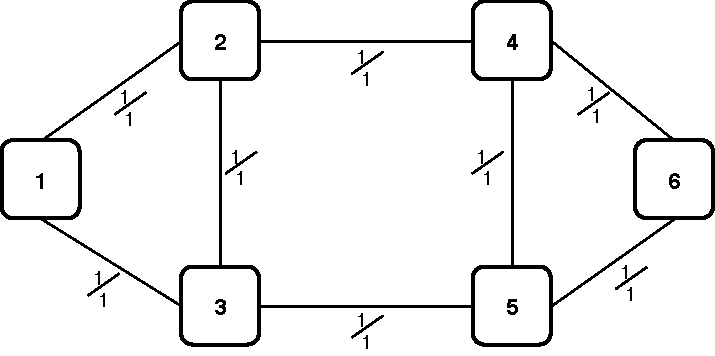
\includegraphics[width=11cm]{sdf/ilp/transparent_survivability/figures/physical_topology}
\caption{Transparent without survivability in high scenario: physical topology after dimensioning.}
\label{physical2_high}
\end{figure}

\vspace{15pt}
\begin{figure}[h!]
\centering
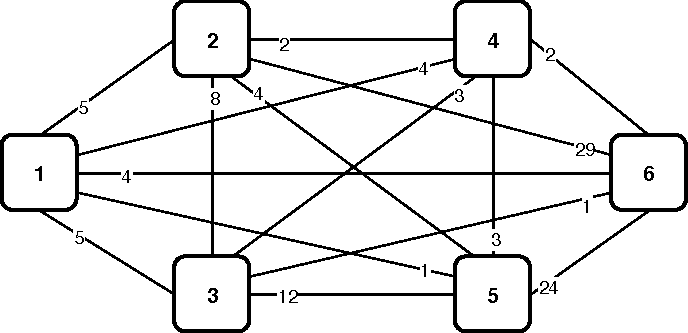
\includegraphics[width=11cm]{sdf/ilp/transparent_survivability/figures/optical_topology_high}
\caption{Transparent without survivability in high scenario: optical topology after dimensioning.}
\label{optical2_high}
\end{figure}

\newpage
In table \ref{link_transp_surv_ref_high} we can see the number of optical channels calculated using \ref{Capex_Link} and \ref{ILPOpaque_CAPEX} and the number of amplifiers for each link calculated using \ref{Capex_amplifiers}.\\

\begin{table}[h!]
\centering
\begin{tabular}{|| c | c | c ||}
 \hline
 \multicolumn{3}{|| c ||}{Information regarding links} \\
 \hline
 \hline
 Bidirectional Link & Optical Channels & Amplifiers\\
 \hline
 Node 1 <-> Node 2 & 13 & 4 \\
 Node 1 <-> Node 3 & 6 & 6 \\
 Node 2 <-> Node 3 & 15 & 0 \\
 Node 2 <-> Node 4 & 42 & 6 \\
 Node 3 <-> Node 5 & 18 & 8 \\
 Node 4 <-> Node 5 & 3 & 1 \\
 Node 4 <-> Node 6 & 35 & 7 \\
 Node 5 <-> Node 6 & 25 & 3 \\
 \hline
\end{tabular}
\caption{Table with information regarding links for transparent mode without survivability in high scenario.}
\label{link_transp_surv_ref_high}
\end{table}

In table \ref{node_transp_surv_ref_high} we can see the number of line ports and add ports using \ref{OXC_poxc_transparent} the number of long-reach transponders using \ref{EXC_pexc2_transparent} and the number of tributary ports using \ref{EXC_pexc1_transparent}.\\

\begin{table}[h!]
\centering
\begin{tabular}{|| c | c | c | c | c | c ||}
 \hline
 \multicolumn{6}{|| c ||}{Information regarding nodes} \\
 \hline
 \hline
 \multicolumn{2}{|| c |}{ } & \multicolumn{2}{ c |}{Electrical part} & \multicolumn{2}{ c ||}{Optical part} \\
 \hline
 Node & Resulting Nodal Degree & Tributary Ports & LR Transponders & Add Ports & Line Ports\\
 \hline
 1 & 2 & 580 & 19 & 19 & 19 \\
 2 & 3 & 460 & 48 & 48 & 70 \\
 3 & 3 & 360 & 29 & 29 & 39 \\
 4 & 3 & 400 & 14 & 14 & 80 \\
 5 & 3 & 480 & 44 & 44 & 46 \\
 6 & 2 & 440 & 60 & 60 & 60 \\
\hline
\end{tabular}
\caption{Table with information regarding nodes for transparent mode without survivability in high scenario.}
\label{node_transp_surv_ref_high}
\end{table}

\newpage
Through the information obtained previously on the nodes we can now create tables with detailed information about each node. In each table mentioned below we can see how many ports are connected to a given node and its bit rate, the number of LR transponders and how many ports are assigned to each different bit rate.\\

\begin{table}[h!]
\centering
\begin{tabular}{|| c | c | c ||}
 \hline
 \multicolumn{3}{|| c ||}{Detailed description of Node 1} \\
 \hline
 \hline
 Electrical part & Number of total demands & Bit rate \\ \hline
\multirow{3}{*}{580 tributary ports} & 260 & ODU0 \\
 & 260 & ODU1 \\
 & 60 & ODU2 \\
 \hline
  & Node<--Optical Channels-->Node & Bit rate \\
 \hline
 \multirow{5}{*}{19 LR Transponders} & 1  <---- 5 ---->  2 & \multirow{5}{*}{100 Gbits/s} \\
  & 1  <---- 5 ---->  3 & \\
  & 1  <---- 4 ---->  4 & \\
  & 1  <---- 1 ---->  5 & \\
  & 1  <---- 4 ---->  6 & \\
 \hline
 \hline
 Optical part & Node<--Optical Channels-->Node & Bit rate \\
 \hline
 \multirow{5}{*}{19 add ports} & 1  <---- 5 ---->  2 & \multirow{10}{*}{100 Gbits/s} \\
  & 1  <---- 5 ---->  3 & \\
  & 1  <---- 4 ---->  4 & \\
  & 1  <---- 1 ---->  5 & \\
  & 1  <---- 4 ---->  6 & \\ \cline{1-2}
 \multirow{5}{*}{19 line ports} & 1  <---- 5 ---->  2 & \\
  & 1  <---- 5 ---->  3 & \\
  & 1  <---- 4 ---->  4 & \\
  & 1  <---- 1 ---->  5 & \\
  & 1  <---- 4 ---->  6 & \\
\hline
\end{tabular}
\caption{Transparent without survivability in high scenario: detailed description of node 1. The number of demands is distributed to the various destination nodes, this distribution can be observed in section \ref{high_traffic_scenario}. Regarding the number of line ports when this node is equal to the source, it means that add ports are used, otherwise it means that through ports are used. In this node as we can see there are no through ports.}
\end{table}

\newpage
\begin{table}[h!]
\centering
\begin{tabular}{|| c | c | c ||}
 \hline
 \multicolumn{3}{|| c ||}{Detailed description of Node 2} \\
 \hline
 \hline
 Electrical part & Number of total demands & Bit rate \\ \hline
\multirow{5}{*}{460 tributary ports} & 220 & ODU0 \\
 & 140 & ODU1 \\
 & 40 & ODU2 \\
 & 40 & ODU3 \\
 & 20 & ODU4 \\
 \hline
  & Node<--Optical Channels-->Node & Bit rate \\
 \hline
 \multirow{5}{*}{48 LR Transponders} & 2  <---- 5 ---->  1 & \multirow{5}{*}{100 Gbits/s} \\
  & 2  <---- 8 ---->  3 & \\
  & 2  <---- 2 ---->  4 & \\
  & 2  <---- 4 ---->  5 & \\
  & 2  <---- 29 ---->  6 & \\
 \hline
 \hline
 Optical part & Node<--Optical Channels-->Node & Bit rate \\
 \hline
 \multirow{5}{*}{48 add ports} & 2  <---- 5 ---->  1 & \multirow{13}{*}{100 Gbits/s} \\
  & 2  <---- 8 ---->  3 & \\
  & 2  <---- 2 ---->  4 & \\
  & 2  <---- 4 ---->  5 & \\
  & 2  <---- 29 ---->  6 & \\ \cline{1-2}
 \multirow{8}{*}{70 line ports} & 2  <---- 5 ---->  1 & \\
  & 2  <---- 8 ---->  3 & \\
  & 2  <---- 2 ---->  4 & \\
  & 2  <---- 4 ---->  5 & \\
  & 2  <---- 29 ---->  6 & \\
  & 1  <---- 4 ---->  4 & \\
  & 1  <---- 4 ---->  6 & \\
  & 3  <---- 3 ---->  4 & \\
\hline
\end{tabular}
\caption{Transparent without survivability in high scenario: detailed description of node 2. The number of demands is distributed to the various destination nodes, this distribution can be observed in section \ref{high_traffic_scenario} . Regarding the number of line ports when this node is equal to the source, it means that add ports are used, otherwise it means that through ports are used. In the latter the number of ports is double the number of optical channels.}
\end{table}

\newpage
\begin{table}[h!]
\centering
\begin{tabular}{|| c | c | c ||}
 \hline
 \multicolumn{3}{|| c ||}{Detailed description of Node 3} \\
 \hline
 \hline
 Electrical part & Number of total demands & Bit rate \\ \hline
\multirow{4}{*}{360 tributary ports} & 140 & ODU0 \\
 & 120 & ODU1\\
 & 60 & ODU2\\
 & 40 & ODU3\\
 \hline
  & Node<--Optical Channels-->Node & Bit rate \\
 \hline
 \multirow{5}{*}{29 LR Transponders} & 3  <---- 5 ---->  1 & \multirow{5}{*}{100 Gbits/s} \\
  & 3  <---- 8 ---->  2 & \\
  & 3  <---- 3 ---->  4 & \\
  & 3  <---- 12 ---->  5 & \\
  & 3  <---- 1 ---->  6 & \\
 \hline
 \hline
 Optical part & Node<--Optical Channels-->Node & Bit rate \\
 \hline
 \multirow{5}{*}{29 add ports} & 3  <---- 5 ---->  1 & \multirow{12}{*}{100 Gbits/s} \\
  & 3  <---- 8 ---->  2 & \\
  & 3  <---- 3 ---->  4 & \\
  & 3  <---- 12 ---->  5 & \\
  & 3  <---- 1 ---->  6 & \\ \cline{1-2}
 \multirow{7}{*}{39 line ports} & 3  <---- 5 ---->  1 & \\
  & 3  <---- 8 ---->  2 & \\
  & 3  <---- 3 ---->  4 & \\
  & 3  <---- 12 ---->  5 & \\
  & 3  <---- 1 ---->  6 & \\
  & 1  <---- 1 ---->  5 & \\
  & 2  <---- 4 ---->  5 & \\
\hline
\end{tabular}
\caption{Transparent without survivability in high scenario: detailed description of node 3. The number of demands is distributed to the various destination nodes, this distribution can be observed in section \ref{high_traffic_scenario} . Regarding the number of line ports when this node is equal to the source, it means that add ports are used, otherwise it means that through ports are used. In the latter the number of ports is double the number of optical channels.}
\end{table}

\newpage
\begin{table}[h!]
\centering
\begin{tabular}{|| c | c | c ||}
 \hline
 \multicolumn{3}{|| c ||}{Detailed description of Node 4} \\
 \hline
 \hline
 Electrical part & Number of total demands & Bit rate \\ \hline
\multirow{3}{*}{400 tributary ports} & 140 & ODU0 \\
 & 200 & ODU1 \\
 & 60 & ODU2 \\
 \hline
  & Node<--Optical Channels-->Node & Bit rate \\
 \hline
 \multirow{5}{*}{14 LR Transponders} & 4  <---- 4 ---->  1 & \multirow{5}{*}{100 Gbits/s} \\
  & 4  <---- 2 ---->  2 & \\
  & 4  <---- 3 ---->  3 & \\
  & 4  <---- 3 ---->  5 & \\
  & 4  <---- 2 ---->  6 & \\
 \hline
 \hline
 Optical part & Node<--Optical Channels-->Node & Bit rate \\
 \hline
 \multirow{5}{*}{14 add ports} & 4  <---- 4 ---->  1 & \multirow{12}{*}{100 Gbits/s} \\
  & 4  <---- 2 ---->  2 & \\
  & 4  <---- 3 ---->  3 & \\
  & 4  <---- 3 ---->  5 & \\
  & 4  <---- 2 ---->  6 & \\ \cline{1-2}
 \multirow{7}{*}{80 line ports} & 4  <---- 4 ---->  1 & \\
  & 4  <---- 2 ---->  2 & \\
  & 4  <---- 3 ---->  3 & \\
  & 4  <---- 3 ---->  5 & \\
  & 4  <---- 2 ---->  6 & \\
  & 1  <---- 4 ---->  6 & \\
  & 2  <---- 29 ---->  6 & \\
\hline
\end{tabular}
\caption{Transparent without survivability in high scenario: detailed description of node 4. The number of demands is distributed to the various destination nodes, this distribution can be observed in section \ref{high_traffic_scenario} . Regarding the number of line ports when this node is equal to the source, it means that add ports are used, otherwise it means that through ports are used. In the latter the number of ports is double the number of optical channels.}
\end{table}

\newpage
\begin{table}[h!]
\centering
\begin{tabular}{|| c | c | c ||}
 \hline
 \multicolumn{3}{|| c ||}{Detailed description of Node 5} \\
 \hline
 \hline
 Electrical part & Number of total demands & Bit rate \\ \hline
\multirow{5}{*}{480 tributary ports} & 280 & ODU0 \\
 & 80 & ODU1 \\
 & 80 & ODU2 \\
 & 20 & ODU3 \\
 & 20 & ODU4 \\
 \hline
  & Node<--Optical Channels-->Node & Bit rate \\
 \hline
 \multirow{5}{*}{44 LR Transponders} & 5  <---- 1 ---->  1 & \multirow{5}{*}{100 Gbits/s} \\
  & 5  <---- 4 ---->  2 & \\
  & 5  <---- 12 ---->  3 & \\
  & 5  <---- 3 ---->  4 & \\
  & 5  <---- 24 ---->  6 & \\
 \hline
 \hline
 Optical part & Node<--Optical Channels-->Node & Bit rate \\
 \hline
 \multirow{5}{*}{44 add ports} & 5  <---- 1 ---->  1 & \multirow{11}{*}{100 Gbits/s} \\
  & 5  <---- 4 ---->  2 & \\
  & 5  <---- 12 ---->  3 & \\
  & 5  <---- 3 ---->  4 & \\
  & 5  <---- 24 ---->  6 & \\ \cline{1-2}
 \multirow{6}{*}{46 line ports} & 5  <---- 1 ---->  1 & \\
  & 5  <---- 4 ---->  2 & \\
  & 5  <---- 12 ---->  3 & \\
  & 5  <---- 3 ---->  4 & \\
  & 5  <---- 24 ---->  6 & \\
  & 3  <---- 1 ---->  6 & \\
\hline
\end{tabular}
\caption{Transparent without survivability in high scenario: detailed description of node 5. The number of demands is distributed to the various destination nodes, this distribution can be observed in section \ref{high_traffic_scenario} . Regarding the number of line ports when this node is equal to the source, it means that add ports are used, otherwise it means that through ports are used. In the latter the number of ports is double the number of optical channels.}
\end{table}

\newpage
\begin{table}[h!]
\centering
\begin{tabular}{|| c | c | c ||}
 \hline
 \multicolumn{3}{|| c ||}{Detailed description of Node 6} \\
 \hline
 \hline
 Electrical part & Number of total demands & Bit rate \\ \hline
\multirow{5}{*}{440 tributary ports} & 160 & ODU0 \\
 & 200 & ODU1 \\
 & 20 & ODU2 \\
 & 20 & ODU3 \\
 & 40 & ODU4 \\
 \hline
  & Node<--Optical Channels-->Node & Bit rate \\
 \hline
 \multirow{5}{*}{60 LR Transponders} & 6  <---- 4 ---->  1 & \multirow{5}{*}{100 Gbits/s} \\
  & 6  <---- 29 ---->  2 & \\
  & 6  <---- 1 ---->  3 & \\
  & 6  <---- 2 ---->  4 & \\
  & 6  <---- 24 ---->  5 & \\
 \hline
 \hline
 Optical part & Node<--Optical Channels-->Node & Bit rate \\
 \hline
 \multirow{5}{*}{60 add ports} & 6  <---- 4 ---->  1 & \multirow{10}{*}{100 Gbits/s} \\
  & 6  <---- 29 ---->  2 & \\
  & 6  <---- 1 ---->  3 & \\
  & 6  <---- 2 ---->  4 & \\
  & 6  <---- 24 ---->  5 & \\ \cline{1-2}
 \multirow{5}{*}{60 line ports} & 6  <---- 4 ---->  1 & \\
  & 6  <---- 29 ---->  2 & \\
  & 6  <---- 1 ---->  3 & \\
  & 6  <---- 2 ---->  4 & \\
  & 6  <---- 24 ---->  5 & \\
\hline
\end{tabular}
\caption{Transparent without survivability in high scenario: detailed description of node 6. The number of demands is distributed to the various destination nodes, this distribution can be observed in section \ref{high_traffic_scenario}. Regarding the number of line ports when this node is equal to the source, it means that add ports are used, otherwise it means that through ports are used. In this node as we can see there are no through ports.}
\end{table}

\vspace{13pt}
Now, in next page, let's focus on the routing information in table \ref{path_transp_surv_ref_high}. These paths are bidirectional so the path from one node to another is the same path in the opposite direction.\\
\newpage
\begin{table}[h!]
\centering
\begin{tabular}{|| c | c | c | c | c | c | c | c ||}
 \hline
 \multicolumn{8}{|| c ||}{Routing} \\
 \hline
 \hline
 o & d & Links & ODU0 & ODU1 & ODU2 & ODU3 & ODU4 \\
 \hline
 1 & 2 & \{(1,2)\} & 100 & 40 & 20 & 0 & 0 \\ \hline
 1 & 3 & \{(1,3)\} & 20 & 80 & 20 & 0 & 0\\ \hline
 1 & 4 & \{(1,2),(2,4)\} & 60 & 40 & 20 & 0 & 0\\ \hline
 1 & 5 & \{(1,3),(3,5)\} & 20 & 0 & 0 & 0 & 0\\ \hline
 1 & 6 & \{(1,2),(2,4),(4,6)\} & 60 & 100 & 0 & 0 & 0\\ \hline
 2 & 3 & \{(2,3)\} & 0 & 0 & 0 & 20 & 0 \\ \hline
 2 & 4 & \{(2,4)\} & 20 & 60 & 0 & 0 & 0\\ \hline
 2 & 5 & \{(2,3),(3,5)\} & 100 & 20 & 20 & 0 & 0 \\ \hline
 2 & 6 & \{(2,4),(4,6)\} & 0 & 20 & 0 & 20 & 20 \\ \hline
 3 & 4 & \{(3,2),(2,4)\} & 20 & 20 & 20 & 0 & 0 \\ \hline
 3 & 5 & \{(3,5)\} & 80 & 20 & 20 & 20 & 0 \\ \hline
 3 & 6 & \{(3,5),(5,6)\} & 20 & 0 & 0 & 0 & 0\\ \hline
 4 & 5 & \{(4,5)\} & 20 & 20 & 20 & 0 & 0\\ \hline
 4 & 6 & \{(4,6)\} & 20 & 60 & 0 & 0 & 0\\ \hline
 5 & 6 & \{(5,6)\} & 60 & 20 & 20 & 0 & 20\\
 \hline
\end{tabular}
\caption{Transparent without survivability in high scenario: description of routing.}
\label{path_transp_surv_ref_high}
\end{table}

Finally and most importantly through table \ref{scripttransp_surv_ref_high} we can see the CAPEX result for this model. This value is obtained using equation \ref{ILPOpaque_CAPEX} and all of the constraints mentioned above.\\

\begin{table}[h!]
\centering
\begin{tabular}{||c|c|c|c|c|c|c||}
 \hline
 \multicolumn{7}{||c||}{CAPEX of the Network} \\
 \hline
 \hline
 \multicolumn{3}{||c|}{}& Quantity & Unit Price & Cost & Total \\
 \hline
 \multirow{3}{*}{\makecell{Link \\ Cost}} &\multicolumn{2}{c|}{OLTs}&16&15 000 \euro&240 000 \euro&\multirow{3}{*}{157 520 000 \euro} \\ \cline{2-6}
 &\multicolumn{2}{c|}{100 Gbits/s Transceivers}&314&5 000 \euro/Gbit/s&157 000 000 \euro& \\ \cline{2-6}
 &\multicolumn{2}{c|}{Amplifiers}&70&4 000 \euro&280 000 \euro& \\
 \hline
 \multirow{10}{*}{\makecell{Node \\ Cost}} &\multirow{7}{*}{Electrical}&EXCs&6&10 000 \euro&60 000 \euro&\multirow{10}{*}{22 951 800 \euro}\\ \cline{3-6}
 & &ODU0 Ports&1 200&10 \euro/port&12 000 \euro& \\ \cline{3-6}
 & &ODU1 Ports&1 000&15 \euro/port&15 000 \euro& \\ \cline{3-6}
 & &ODU2 Ports&320&30 \euro/port&9 600 \euro& \\ \cline{3-6}
 & &ODU3 Ports&120&60 \euro/port&7 200 \euro& \\ \cline{3-6}
 & &ODU4 Ports&80&100 \euro/port&8 000 \euro& \\ \cline{3-6}
 & &Transponders&214&100 000 \euro/port&21 400 000 \euro&\\ \cline{2-6}
 & \multirow{3}{*}{Optical}&OXCs&6&20 000 \euro&120 000 \euro& \\ \cline{3-6}
 & &Line Ports&314&2 500 \euro/port&785 000 \euro& \\ \cline{3-6}
 & &Add Ports&214&2 500 \euro/port&535 000 \euro& \\
 \hline
 \multicolumn{6}{||c|}{Total Network Cost} & 180 471 800 \euro \\
\hline
\end{tabular}
\caption{Transparent without survivability in high scenario: detailed description of CAPEX for this scenario.}
\label{scripttransp_surv_ref_high}
\end{table}

\newpage
\subsection{Conclusions}

Once we have obtained the results for all the scenarios we will now draw some conclusions about these results. For a better analysis of the results will be created the table \ref{table_comparative_transp_surv} with the number of line ports and add ports of the optical part, the tributary ports, the transponders and transceivers because they are important values for the cost of CAPEX, the cost of links, the cost of nodes and finally the cost of CAPEX.\\

\begin{table}[h!]
\centering
\begin{tabular}{| c | c | c | c |}
 \hline
  & Low Traffic & Medium Traffic  & High Traffic \\
 \hline\hline
 Traffic (Gbit/s) & 500 & 5 000 & 10 000 \\ \hline
 Number of Add ports & 34 & 114 & 214 \\ \hline
 Number of Line ports & 52 & 168 & 314 \\ \hline
 Number of Tributary ports & 136 & 1 360 & 2 720 \\ \hline
 Number of Transceivers & 52 & 168 & 314 \\ \hline
 Number of Transponders & 34 & 114 & 214 \\ \hline
 Link Cost & 26 520 000 \euro & 84 520 000 \euro & 157 520 000 \euro \\ \hline
 Node Cost & 3 797 590 \euro & 12 310 900 \euro & 22 951 800 \euro \\ \hline
 CAPEX & \textbf{30 317 590 \euro} & \textbf{96 830 900 \euro} & \textbf{180 471 800 \euro} \\ \hline
 CAPEX/Gbit/s & \textbf{60 635 \euro/Gbit/s} & \textbf{19 366 \euro/Gbit/s} & \textbf{18 047 \euro/Gbit/s}\\
 \hline
\end{tabular}
\caption{Transparent without survivability: Table with the various CAPEX values obtained in the different traffic scenarios.}
\label{table_comparative_transp_surv}
\end{table}

Looking at the previous table we can make some comparisons between the several scenarios:

\begin{itemize}
  \item Comparing the low traffic with the others, we can see that once again the number of transceivers is lower than expected, reducing the number of components and consequently the CAPEX of the network.
  \item Comparing the medium traffic with the high traffic we can see that the increase of the factor and the final cost are very close but still inferior. This happens because the real number of the transceivers is closer to the expected.
  \item Comparing the CAPEX cost per bit we can see that in the low traffic the cost is higher than the medium and high traffic. This happens because the higher the traffic, the lower CAPEX/Gbit/s will be. We can see that in medium and high traffic the results tend to be one closer and lower value.
\end{itemize}

